%
% LO, Li-yu 
%

\documentclass[a4paper,12pt]{article}

\usepackage{graphicx}
\usepackage[english]{babel}
\usepackage[]{amsmath}
\usepackage{amsfonts}
\usepackage{mathtools}
\usepackage{amssymb}
\usepackage[a4paper, portrait, margin=0.8in]{geometry}
\usepackage{hyperref}
\usepackage{algorithm,algpseudocode}
\usepackage{indentfirst}
\usepackage{soul}
\usepackage{color}
% \usepackage{subfigure}
\usepackage{titling}
% \usepackage{subcaption}
\usepackage{subfig}
\usepackage[labelfont=bf, justification=justified]{caption}
% \usepackage[demo]{graphicx}% Remove demo option in real document


\setlength{\droptitle}{-4em}   % This is your set screw

\begin{document}
%
   \title{\textbf{COMP5212 Machine Learning} \\  
   Programming Homework 1}
   
   \author{LO, Li-yu \\ 20997405 \\ e-mail: lloac@connect.hkust.hk}
   \date{\today}
   \maketitle

\vspace*{-1.2cm}
\section*{Abstract}
\vspace*{-0.4cm}
In this assignment, a binary classification model based on 
(1) \textbf{Linear Logistic Regression (LLR)} and 
(2) \textbf{Linear Support Vector Machine (LSVM)} is trained.
In particular, we perform the the classification on the \textbf{0} and \textbf{1} 
subclass of the MNIST digit dataset, whilst adopting PyTorch library as our main 
programming framework. Below then reports the training results.
\section*{General Training Results}
\vspace*{-0.4cm}
Below first present the training results of each model by plotting the 
\textit{batch-averaged loss versus epochs}, 
in which LLR and LSVM utilize both Stochastic Gradient Descent (SGD) 
and Stochastic Gradient Descent Momentum (SGD-M) optimizer. 
Also note that in the below cases, we set $learning \; rate \; \alpha=0.01$
and $epoch=20$.
For SGD-M, we set momentum beta coefficient with $\beta=0.9$.
\vspace*{-0.6cm}
\begin{figure}[!htb]
   \captionsetup[subfigure]{justification=centering}
   \centering
   \subfloat[][Linear Logistic Regression \\ w/ Stochastic Gradient Descent]
   {%
      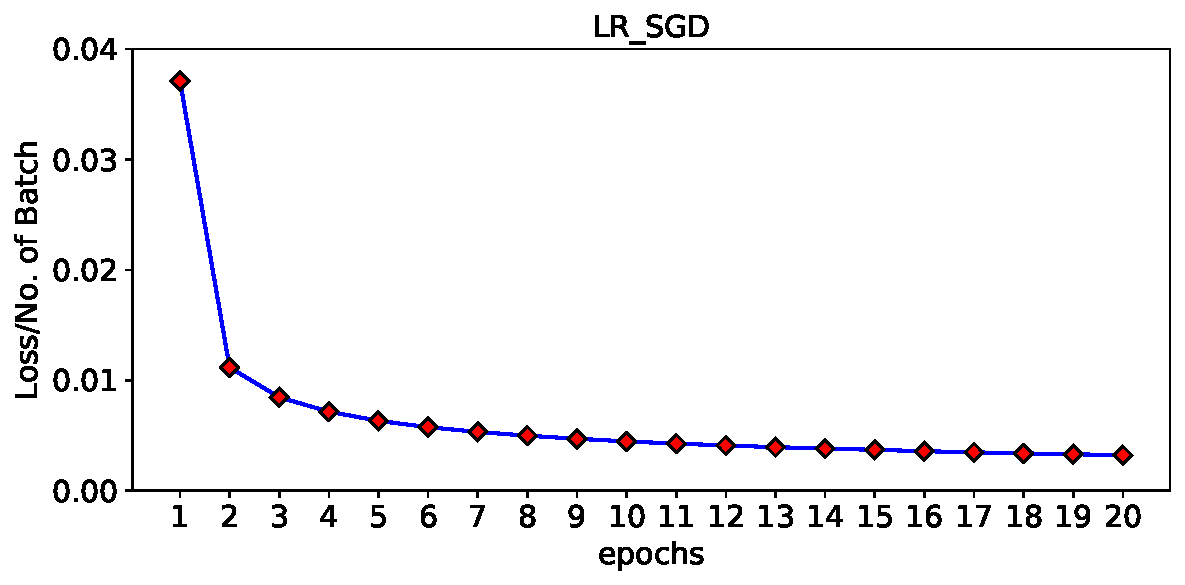
\includegraphics[width=0.45\textwidth]{./results/LR_SGD.pdf}%
      \label{fig:llr_sgd}
   }%
   \hspace{1cm}%
   \subfloat[][Linear Logistic Regression \\ w/ Stochastic Gradient Descent Momentum]
   {%
      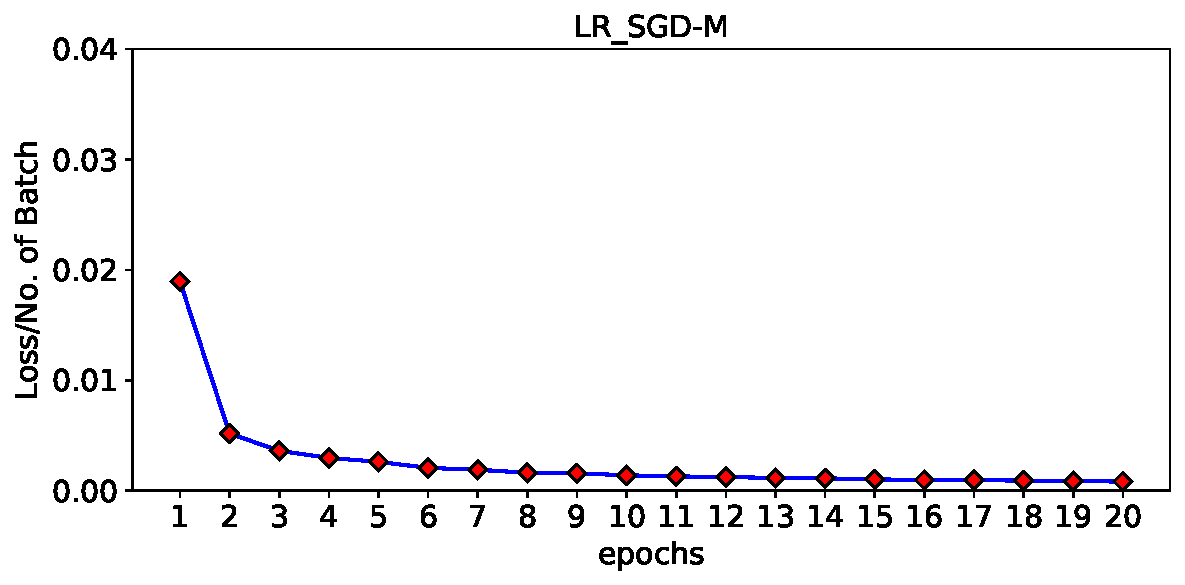
\includegraphics[width=0.45\textwidth]{./results/LR_SGD-M.pdf}%
      \label{fig:llr_sgdm}
   }
   \hspace{1cm}%
   \subfloat[][Linear Support Vector Machine \\ w/ Stochastic Gradient Descent]
   {%
      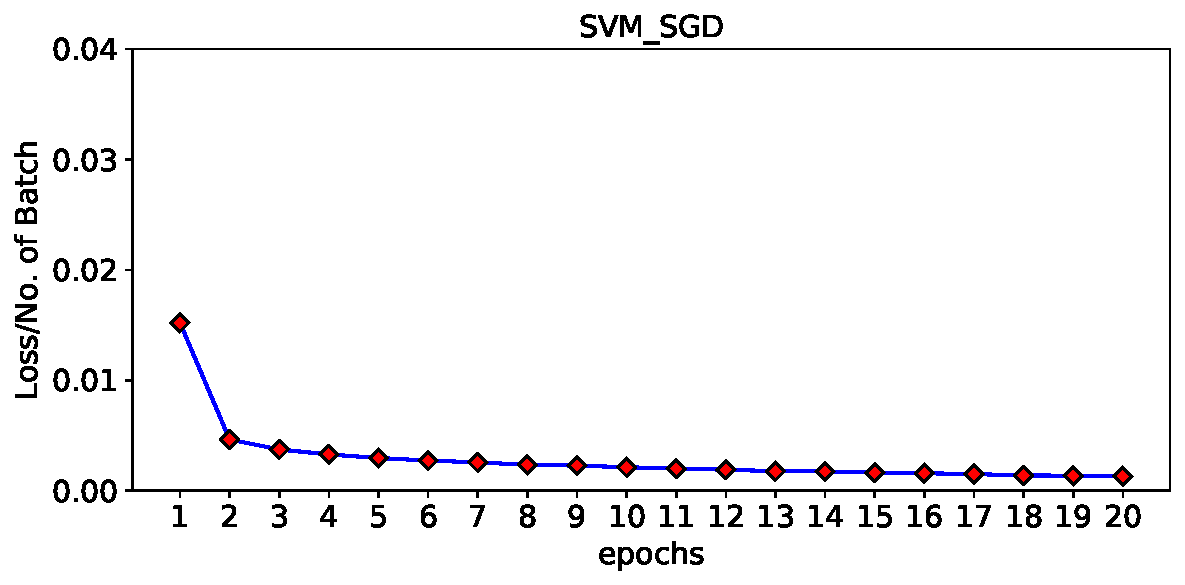
\includegraphics[width=0.45\textwidth]{./results/SVM_SGD.pdf}%
      \label{fig:svm_sgd}
   }%
   \hspace{1cm}%
   \subfloat[Linear Support Vector Machine \\ w/ Stochastic Gradient Descent Momentum]
   {%
      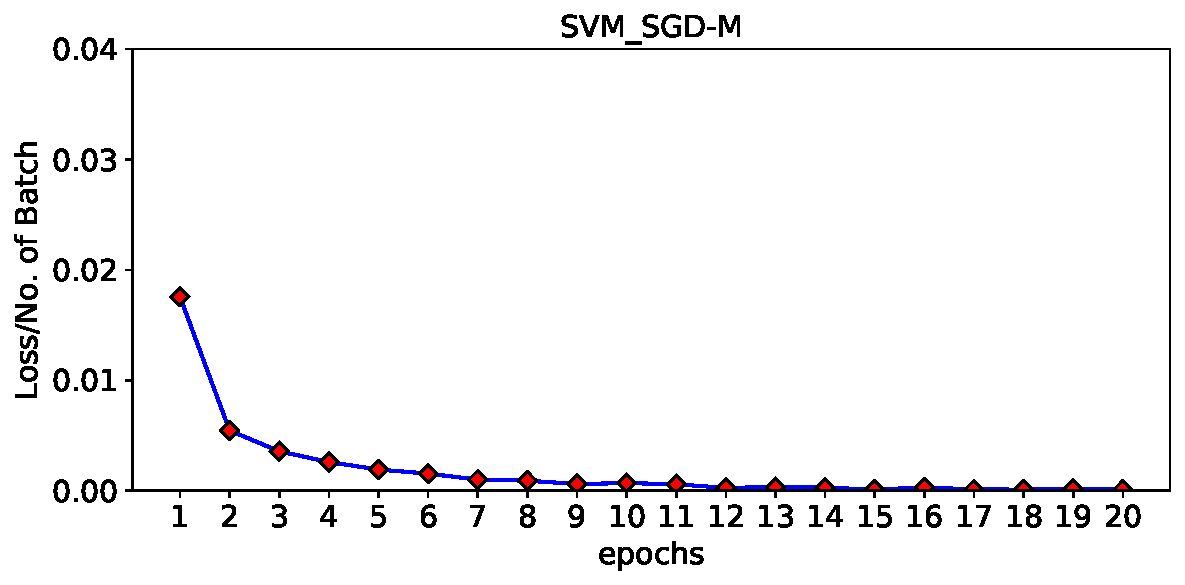
\includegraphics[width=0.45\textwidth]{./results/SVM_SGD-M.pdf}%
      \label{fig:svm_sgdm}
   }
   \caption{Training results of different cases.}
\end{figure}
% \vspace*{-0.6cm}
\section*{Testing Accuracy}
\vspace*{-0.4cm}
We also report the \textit{accuracy versus epoch} retrieved from the testing dataset,
where plots of the 4 cases are shown. 
It can be observed that for all 4 cases, all models swiftly approach
to accuracy of over 99 \%, which show extremely high performance in the binary classification task. 
\begin{figure}[!htb]
   \captionsetup[subfigure]{justification=centering}
   \centering
   \subfloat[][Linear Logistic Regression \\ w/ Stochastic Gradient Descent]
   {%
      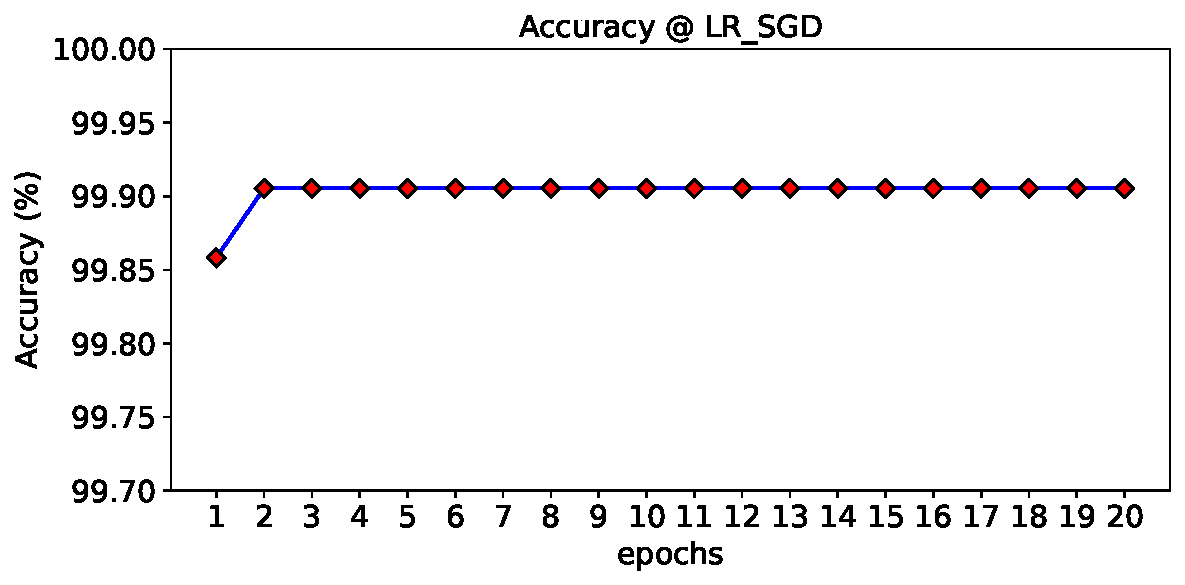
\includegraphics[width=0.225\textwidth]{./results/LR_SGD_accuracy.pdf}%
      \label{fig:llr_acc_sgd}
   }%
   % \label{fig:llr_sgd}
   \hspace{0.5cm}%
   \subfloat[][Linear Logistic Regression \\ w/ Stochastic Gradient Descent Momentum]
   {%
      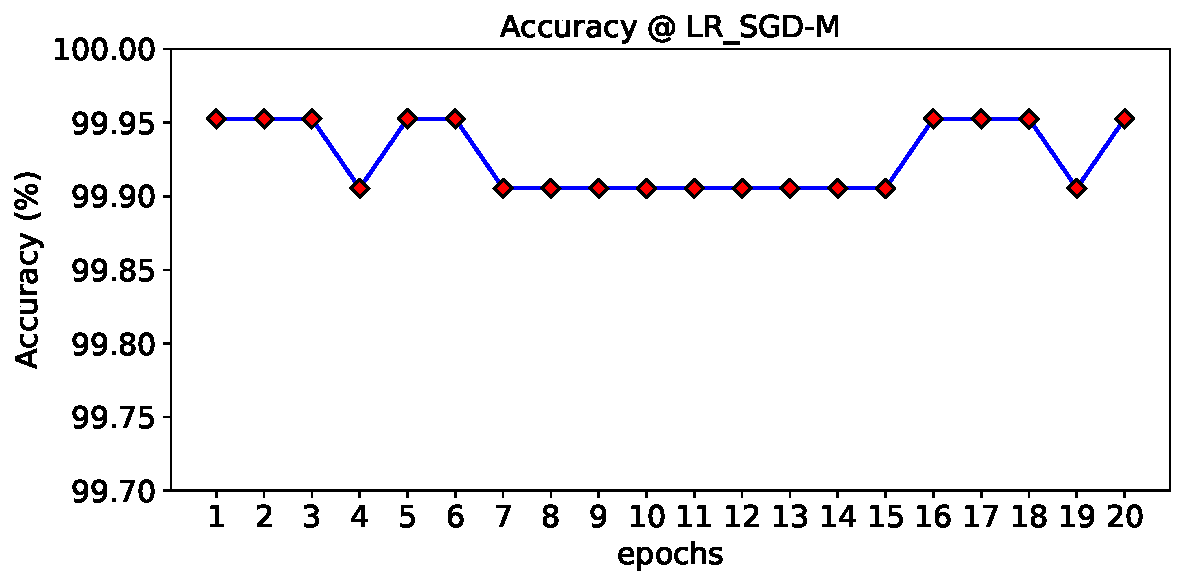
\includegraphics[width=0.225\textwidth]{./results/LR_SGD-M_accuracy.pdf}%
   }
   % \label{fig:llr_sgdm} 
   \hspace{0.5cm}%
   \subfloat[][Linear Support Vector Machine \\ w/ Stochastic Gradient Descent]
   {%
      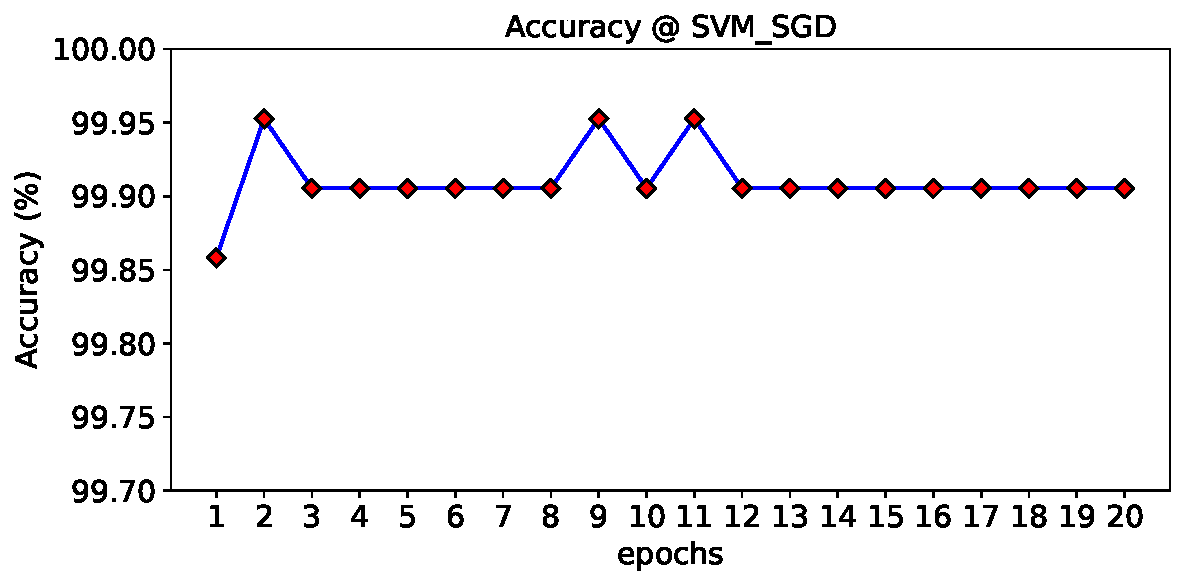
\includegraphics[width=0.225\textwidth]{./results/SVM_SGD_accuracy.pdf}%
   }%
   \hspace{0.5cm}%
   \subfloat[Linear Support Vector Machine \\ w/ Stochastic Gradient Descent Momentum]
   {%
      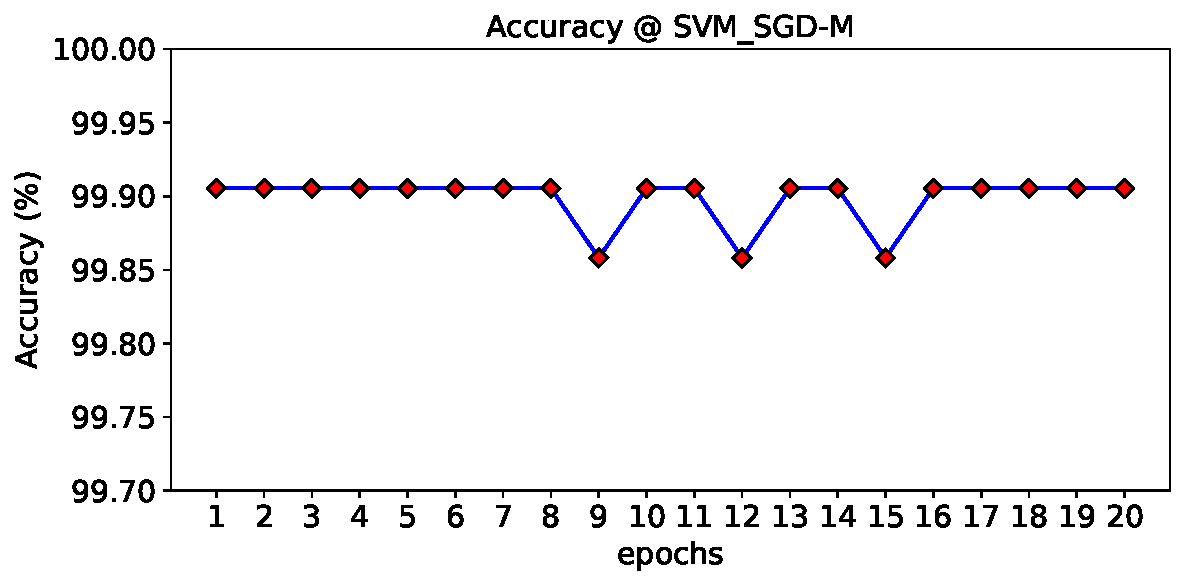
\includegraphics[width=0.225\textwidth]{./results/SVM_SGD-M_accuracy.pdf}%
   }
   \caption{Model accuracy versus epochs.}
\end{figure}
\section*{On SGD v. SGD-M}
\vspace*{-0.4cm}
By referring to figure \ref{fig:llr_sgd} and \ref{fig:llr_sgdm}, 
or figure \ref{fig:svm_sgd} and \ref{fig:svm_sgdm}, it can be easily seen that 
with momentum, in which previous gradients information are taken into consideration,
the training process could converge faster.
Although in the case of support vector machine, 
i.e., figure \ref{fig:svm_sgd} and \ref{fig:svm_sgdm},
SGD with momentum converge slightly slower at first,
yet, after 5 epochs, it could be observed that it further suppress the loss,
leading to a more optimal minimum region.
\section*{On Learning Rate $\alpha$ Settings}
\vspace*{-0.4cm}
The last section presents the analysis on hyperparameter settings of learning rate $\alpha$.
To fixate same comparison condition, we use Linear Logistic Regression
with Stochastic Gradient Descent for analysis.
In addition, for $\alpha$, we set $\alpha=[0.2,0.1,0.01,0.001,0.0001]$.
Below plots the final comparative results.
\begin{figure}[!htb]
   \captionsetup[subfigure]{justification=centering}
   \centering
   \subfloat[][Linear Logistic Regression \\ w/ Different $\alpha$]
   {%
      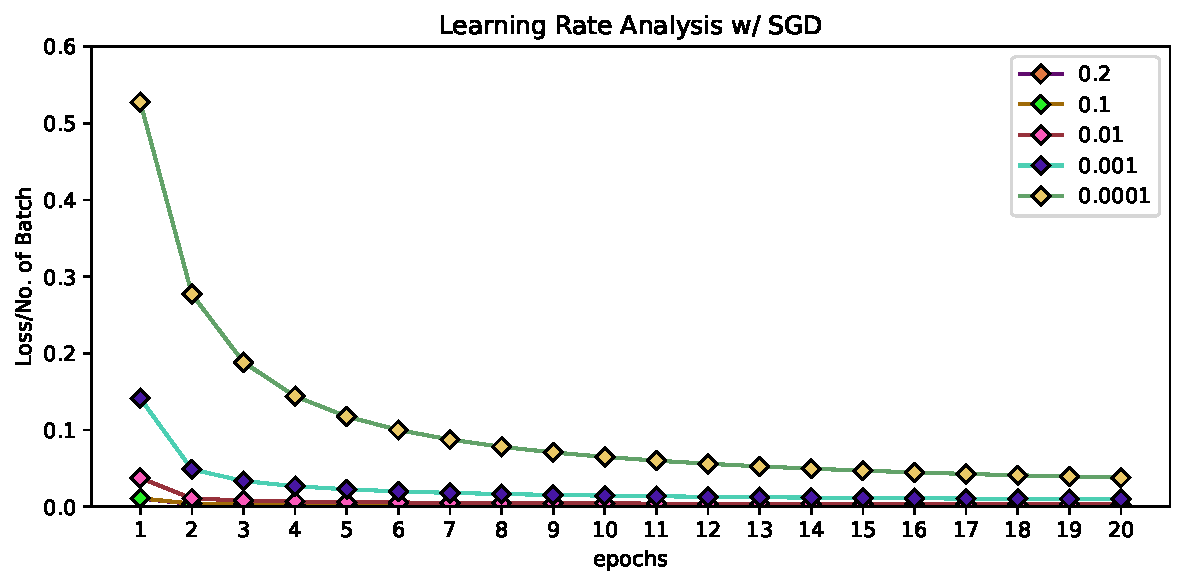
\includegraphics[width=0.45\textwidth]{./results/LLR_SGD_step_size_analy.pdf}%
      \label{fig:analysis}
   }%
   \hspace{1cm}%
   \subfloat[][Zoomed-in Linear Logistic Regression \\ w/ Different $\alpha$]
   {%
      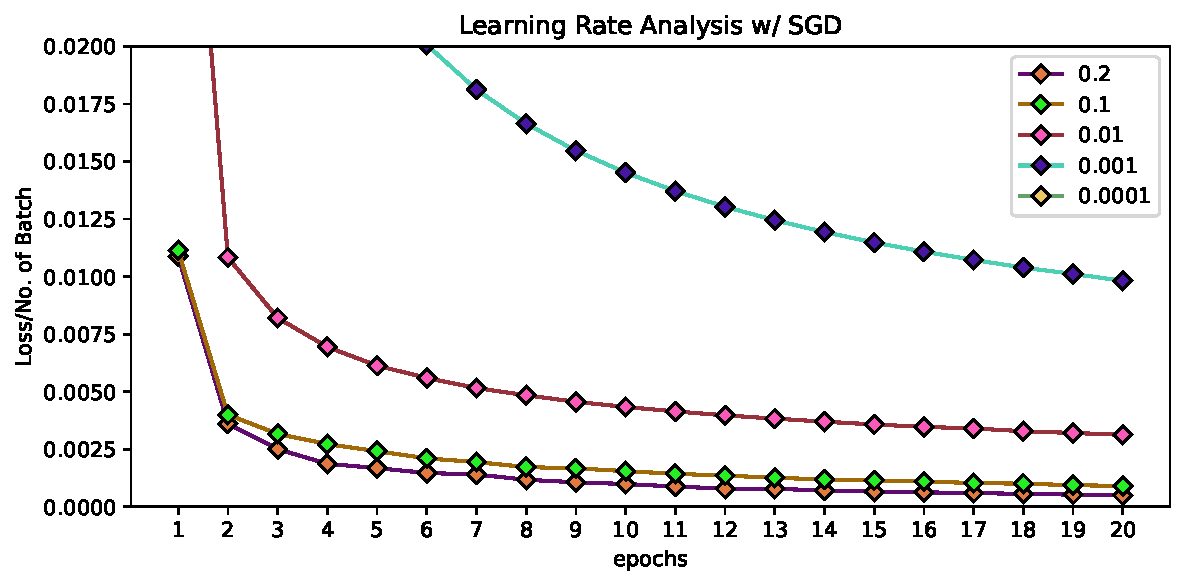
\includegraphics[width=0.45\textwidth]{./results/LLR_SGD_step_size_analy_zoomin.pdf}%
      \label{fig:analysis_zoomin}
   }
   \caption{Learning rate analysis.}
\end{figure}
\noindent From above, it can be easily concluded that with larger learning rate, 
the model could converge faster, as we are moving our model in the downward slope 
with larger step. 
Nevertheless, it is also discovered that, when setting $\alpha$ with a larger scale,
say $\alpha=0.9$, the learning process could result in disastrous failure,
since such settings could lead to huge divergence.
For instance, weights could be updated by large values with large $\alpha$, 
and hence leading to an exploding gradients;
then, the training will end up diverging at an exponentially increasing rate.
\bibliographystyle{IEEEtran}
% \bibliography{references}

\end{document}

